\documentclass[aps,prl,reprint]{revtex4-1}
\usepackage{blindtext}

\usepackage{amsmath}
\usepackage{graphicx}
\usepackage{commath}
\usepackage{siunitx}

\usepackage[b]{esvect}

\newcommand{\de}{\mathrm{d}}

\begin{document}
\title{Homework 1}
\author{Xueqi Li}
\noaffiliation
% \date{Feb 4, 2017}
% \email{xueqi.li@stonybrook.edu}

% \begin{abstract}
% Consider a vector (given with respect to a fixed Cartesian basis). Here $t$ means time.
% \[
% \vv{r}(t) = \sin(\pi t)\hat{x} + \cos(\pi t)\hat{y} - \sqrt{7}\hat{z}
% \]
% \end{abstract}

\maketitle

\section{Problem 2.16}
A golfer hits his ball with speed $v_0$ at an angle $\theta$ above the hoizotal ground. Assuming that the angle $\theta$ is fixed and that air resistance can be neglected, what is the minimul speed $v_0$ for wich the ball will clear a wall of hight $h$, a distance $d$ away? Your solution should get into trouble if the angle $\theta$ is such taht $\tan\theta < \frac{h}{d}$. Explain. What is the minimum speed if $\theta = \ang{25}$, $d = 50\si{\metre}$, and $h = 2 \si{\metre}$.
\subsection{Solution}
Since air resistance can be neglected, we could have $\vv{F}= m \ddot{\vv{r}} = -mg\hat{y}$. We can see that $v_x(0) = \cos\theta v$ and $v_y(0) = \sin\theta v$. Thus we have following equations:
\begin{eqnarray*}
    \frac{\de r_x}{\de t} = v_x(0) \\
    \frac{\de^2 r_y}{\de t^2} = -g
\end{eqnarray*}
Easy to find
\begin{eqnarray*}
    r_x &=& \int v_x(0) \de t = v_x(0) t + r_x(0)\\
    \frac{\de r_y}{\de t} &=& \int -g \de t = -gt + v_y(0)\\
    r_y &=& \int -gt \de t + \int v_y(0)\de t \\
        &=& -g \int t \de t + v_y(0) t + r_y(0) \\
        &=& -g \frac{t^2}{2} + v_y(0) t + r_y(0)
\end{eqnarray*}
Let $r(0) = (0,0)$, we could have:
\begin{eqnarray*}
    r_x &=& v_x(0) t\\
    r_y &=& -g \frac{t^2}{2} + v_y(0) t
\end{eqnarray*}
Now we can plug back $v$ and $\theta$, we have:
\begin{eqnarray*}
    r_x &=& \cos\theta v t\\
    r_y &=& -g \frac{t^2}{2} + \sin\theta v t
\end{eqnarray*}
From the first euqation we can find the time $t$ that the golfer reach the ground when $r_x = d$. And this give us $t = \frac{d}{\cos\theta v}$.

Now plug it in to 2nd equation:
\begin{eqnarray*}
r_y &=& -g \frac{t^2}{2} + \sin\theta v \frac{d}{\cos\theta v} \\
r_y &=& -g \frac{d^2}{2\cos^2\theta v^2} + \tan\theta d
\end{eqnarray*}
In our case, we wish $r_y > h$. Let look at the case where $\theta = \frac{h}{d}$. We have;
\begin{eqnarray*}
r_y &=& -g \frac{d^2}{2\cos^2\theta v^2} + \frac{h}{d} d \\
h &<& -g \frac{d^2}{2\cos^2\theta v^2} + h
\end{eqnarray*}
Notice that $g \frac{d^2}{2\cos^2\theta v^2}$ always larger than zero. Thus for any t it is not possable to have $h < h - a$ where $a > 0$. Thus this means it is not possable to clear such a wall.

When $\tan\theta < \frac{h}{d}$. $\tan\theta d < \frac{h}{d} d$, we will have:
\[
h < -a + h< -a + \tan\theta d
\]
where $a > 0$. This means right side is always smaller than $h$. It is not possable to clear such a wall.

Now plug in the numbers in to equation, we have:
\[
2 < -10 \frac{50^2}{2\cos^2\ang{25} v^2} + 50 \tan\ang{25} 
\]
Solve the equation we have the min $v = 26.72$m/s.







% Since air resistance can be neglected, we could have $\vv{F}= m \ddot{\vv{r}} = -mg\hat{y}$. We can see that $v_x(0) = \cos\theta v$ and $v_y(0) = \sin\theta v$. Thus we have following equations:
% \begin{eqnarray*}
%     \frac{\de r_x}{\de t} = v_x(0) \\
%     \frac{\de^2 r_y}{\de t^2} = -g
% \end{eqnarray*}
% Easy to find
% \begin{eqnarray*}
%     r_x &=& \int v_x(0) \de t = v_x(0) t + r_x(0)\\
%     \frac{\de r_y}{\de t} &=& \int -g \de t = -gt + v_y(0)\\
%     r_y &=& \int -gt \de t + \int v_y(0)\de t \\
%         &=& -g \int t \de t + v_y(0) t + r_y(0) \\
%         &=& -g \frac{t^2}{2} + v_y(0) t + r_y(0)
% \end{eqnarray*}
% Let $r(0) = (0,0)$, we could have:
% \begin{eqnarray*}
%     r_x &=& v_x(0) t\\
%     r_y &=& -g \frac{t^2}{2} + v_y(0) t
% \end{eqnarray*}
% When $r_y$ is maximum, $\frac{\de r_y}{\de t} = 0$. Thus we have
% \begin{eqnarray*}
% gt &=& v_y(0) \\
% t_{\mathrm{max}} &=& \frac{v_y(0)}{g}
% \end{eqnarray*}
% And we want
% \begin{eqnarray*}
% r_y(t_{\mathrm{max}}) &=& h \\
% r_y(t_{\mathrm{max}}) &=& d
% \end{eqnarray*}
% Thus we can have
% \begin{eqnarray*}
% v_x(0) \frac{v_y(0)}{g} &=& h \\
% -g \frac{(\frac{v_y(0)}{g})^2}{2} + v_y(0) \frac{v_y(0)}{g} &=& d
% \end{eqnarray*}
% Solve the equation, we chould have $v_x(0) = \sqrt{\frac{g}{2d}}h$ and $v_y(0) = \sqrt{2dg}$. Thus we can now solve $\norm{v}$ and $\theta$:
% \begin{eqnarray*}
%     \sqrt{\frac{g}{2d}}h &=& \cos\theta v\\
%     \sqrt{2dg} &=& \sin\theta v
% \end{eqnarray*}
% Solve the equation and we can find $\theta$ and $v(0)$.
% we can find $\tan \theta$ from above equations as
% \begin{eqnarray*}
% \frac{\sqrt{2dg}}{\sqrt{\frac{g}{2d}}h} &=& \tan\theta\\
% \frac{2d}{h} &=& \tan\theta
% \end{eqnarray*}
% Thus we can have $\theta = \arctan\frac{2d}{h}$. Thus we can have $v = \sqrt{(\sqrt{\frac{g}{2d}}h)^2 + (\sqrt{2dg})^2} = \sqrt{\frac{g}{2d}h^2 + 2dg}$.

% Plug the number into the euqation


\section{Problem 2.36}
Consider the following quote from Galileo's \textit{Dialogues Concerning Two New Sciences}:

Aristotle says that ``an iron ball of 100 pounds falling from a height of one hundred cubits reches the ground before a one-pound ball has fallen a single cubit.'' I say taht they arrive at the same time. You find, on making the experiment, that the larger outstrips the smaller by two finger-breadths, that is, when the larger has reached the ground, the other is short of it by two finger-breadths.

We know that the statement attributed to Aristotle is totally worong, but just how close is Galileo's claim that the difference is just ``two finger breadths''?
\begin{enumerate}
    \item Given that the density of iron is about 8\si{\gram\per\centi\metre\cubed}, find the terminal speed of the two iron balls.
    \item Given that a cubit is about 2 feet, use Equation (2.58) to find the time for the heavier ball to land and then the position of the lighter ball at that time. How far apart are they.
\end{enumerate}
\[
y = \frac{v_{\text{ter}}^2}{g} \ln\left[\cosh\frac{gt}{v_{\text{ter}}}\right]
\]
Use quadratic drag and $x = \dot{x}=0$.
\subsection{Solution}
\begin{enumerate}
    \item 100 Pounds is 45kg. We can calculate $V_{100} = 0.0056$m$^3$, giving $r = 0.11$m.Plug the value into equation (2.50) of the book we have $v_\text{ter} = \sqrt{\frac{mg}{\gamma D^2}} = \sqrt{\frac{45\times 10}{0.25\times (2 \times 0.11)^2}} = 192.847$m/s.

    1 Pounds is 0.45kg. Thus we have $V_1 = 0.00005626$m$^3$, giving $r = 0.024$m. Thus we have $v_\text{ter} = \sqrt{\frac{mg}{\gamma D^2}} = \sqrt{\frac{0.45\times 10}{0.25\times (2\times0.024)^2}} = 88.39$m/s.
    \item Using the equation we have for 100 pounds ball:
    \[
        61 = \frac{192.847^2}{10} \ln[\cosh (\frac{10 t}{192.847})]
    \]
    Solve the equation we have t = 3.50s. Now plug it into the euqation for the smaller ball:
    \[
        y = \frac{88.39^2}{10} \ln[\cosh (\frac{10 \times 3.50}{88.39})] = 59.7\mathrm{m}
    \]

    And we can find the difference is 1.3m.
\end{enumerate}

\section{Problem 1}
Consider a body with a cross-sectional area $A$ moving with speed $\norm{v}$ through a fluid with density $\rho$. We showed using dimensional analysis that this gave rise to a drag force proportional to $\rho A \norm{v}^2$.
\begin{enumerate}
    \item At what rate does the body encounter the fluid, that is how much mass per second does it hit?
    \item To accelerate all this fluid to the body’s speed $\norm{v}$, what force needs to be exerted? 

    In reality, the body doesn't accelerate all the fluid it encounters to its own speed, but this gives a rough measure of the drag force. For a sphere, it turns out that the force is about $\frac{\rho A \norm{v}^2}{4}$. In air room temperature and presure (STP), $\rho \approx 1.3\si{\kilo\gram\per\cubic\metre}$
    \item Find the constant c in equation (3.35) of the notes in terms of the diameter $D$ of the sphere. How does this result compare to (2.6) in the book?
\end{enumerate}
\[
\ddot{\vv{r}} = -g\hat{z}-\frac{c}{m}v\vv{v}
\]
\[
\gamma = 0.25\si{\newton\second\squared\per\metre\tothe{4}}
\]
\subsection{Solution}
\begin{enumerate}
    \item When the body encounter the fluid. The volume of the fluid that is been hit is $\int A \norm{v} \de t$. Giveing the rate is $A\norm{v}$ And to find the mass, knowing the dencity, we can find the rate is $A\norm{v}\rho$.
    \item The mass that it accelerate is $A\norm{v}\rho$ pre sec. Thus we have $F = A\norm{v}\rho a$ per sec. We wish to accelerate the fluid to $\norm{v}$ from $0$. Thus we have $a = v$. THus we have $F = F = A\norm{v}^2\rho$.
    \item Knowing the force, we could set up the euqation:
    \[
    \frac{\rho A(t) v^2}{4}m = -g\hat{z}-\frac{c}{m}v\vv{v}
    \]
    where $A = \pi (\sin(\arccos\frac{R-tv}{R})R)^2 = \pi (1-\frac{R-tv}{R})R^2$. Thus we have:
    \[
    \frac{\rho\pi (1-\frac{R-tv}{R})R^2\pi (1-\frac{R-tv}{R})R^2 v^2}{4}m = -g\hat{z}-\frac{c}{m}v\vv{v}
    \]
\end{enumerate}
\section{Problem 2}
For one-dimensional motion along the z-axis, if $F_z = f(z)$ for an arbitrary function $f$, write the general solution relating $v_z$ and $z$ in terms of an integral (hint–multiply the equation through by $v_z \equiv \dot{z}$).
\subsection{Solution}
\begin{eqnarray*}
F_z = f(z) &=& m\ddot{r}_z \\
\frac{\de^2 z}{\de t^2} &=& \frac{f(z)}{m} \\
v_z = \frac{\de z}{\de t} &=& \frac{1}{m}\int f(z)\de t \\
&=& \frac{1}{m}\int_0^d f(z)\de d + v_z(0)
% z &=& \frac{1}{m} \iint f(z) (\de t) ^2
\end{eqnarray*}
\section{Problem 3}
For one-dimensional motion along the z-axis, if $F_z = f(v_z)$ for an arbitrary function $f$, write the general solution relating $t$ and $v_z$ in terms of an integral.
\subsection{Solution}
\begin{eqnarray*}
F_z = f(v_z) &=& m\ddot{r}_z \\
\frac{\de v_z}{\de t} &=& \frac{f(v_z)}{m} \\
\de v_z &=& \frac{f(v_z)}{m}\de t \\
\frac{\de v_z}{f(v_z)} &=& \frac{1}{m} \de t \\
\int \frac{\de v_z}{f(v_z)} &=& \frac{1}{m} t + C \\
\end{eqnarray*}
\section{Problem 4}
For quadratic drag, suppose $\dot{z}(0) = 0$
\begin{enumerate}
    \item What is the initial slope $w_0$ in this case? What is the integration constant A in equation (3.44) of the notes?
    \item The mass falls; after some time, $v_x = -v_z$. Use (3.38) of the note, the definition of the slope $w$, and (3.43) to find what the velocity is. Notice how this simplifies when the drag $c = 0$; what is the physical reason for this?
    \item More generally, use (3.38), the definition of the slop $w$, (3,43), and (3,44) to write down the exact relation between $v_x$ and $v_z$ for arbitrary $\dot{x}_0$ and $\dot{z}_0$ - this is a complicated equation relating $v_z$, $v_z$, $\dot{x}_0$, $\dot{z}_0$.
\end{enumerate}
\subsection{Solution}
\begin{enumerate}
    \item Since $w(0) = \frac{v_z}{v_x} = 0$. We have $A = 0 + \ln(0 + \sqrt{1+0})+\frac{mg}{c\dot{x}_0^2} = \frac{mg}{c\dot{x}_0^2}$.
    \item We could have from (3.38)
    \[
        \dot{w} = -\frac{g}{v_x}
    \]
    and plug it in to (3.43) to have
    \[
        \frac{g^2}{v_x^2} = -\frac{cg}{m}(w\sqrt{1+w^2}+\ln(w+\sqrt{q+w^2})-\frac{mg}{c\dot{x}_0^2})
    \]
    Knowing that $v_x = -v_z$, we could have $w = -1$. Thus we have
    \[
        \frac{g}{v_x^2} = -\frac{c}{m}(-\sqrt{2}+\ln(-1+\sqrt{2})-\frac{mg}{c\dot{x}_0^2})
    \]
    Easy to solve for $v_x$
    \[
        v_x = \sqrt{\frac{mg}{\sqrt{2}c-c\ln(\sqrt{2}-1)+\frac{mg}{\dot{x}_0^2}}}
    \]
    And $v_z = -v_x$.

    When $c = 0$, we can find that $v_x = \sqrt{\frac{mg}{(\frac{mg}{\dot{x}_0^2})}} = x_0$. Physicaly, that is how we solve the problem when air resistance can be neglected, i.e., the velocity in $x$ direction preserve.
    \item We would have:
    \[
    -\frac{g}{v_x} = -\frac{cg}{m}(\frac{v_z}{v_x}\sqrt{1+\frac{v_z^2}{v_x^2}}+\ln[\frac{v_z}{v_x} + \sqrt{1+\frac{v_z^2}{v_x^2}}]-A)
    \]
    where 
    \[
    A = \frac{\dot{z}_0}{\dot{x}_0}\sqrt{1 + \frac{\dot{z}_0^2}{\dot{x}_0^2}} + \ln(\frac{\dot{z}_0}{\dot{x}_0} + \sqrt{1+ \frac{\dot{z}_0^2}{\dot{x}_0^2}})+\frac{mg}{c\dot{x}^2_0}
    \]
\end{enumerate}
%\begin{center}
% 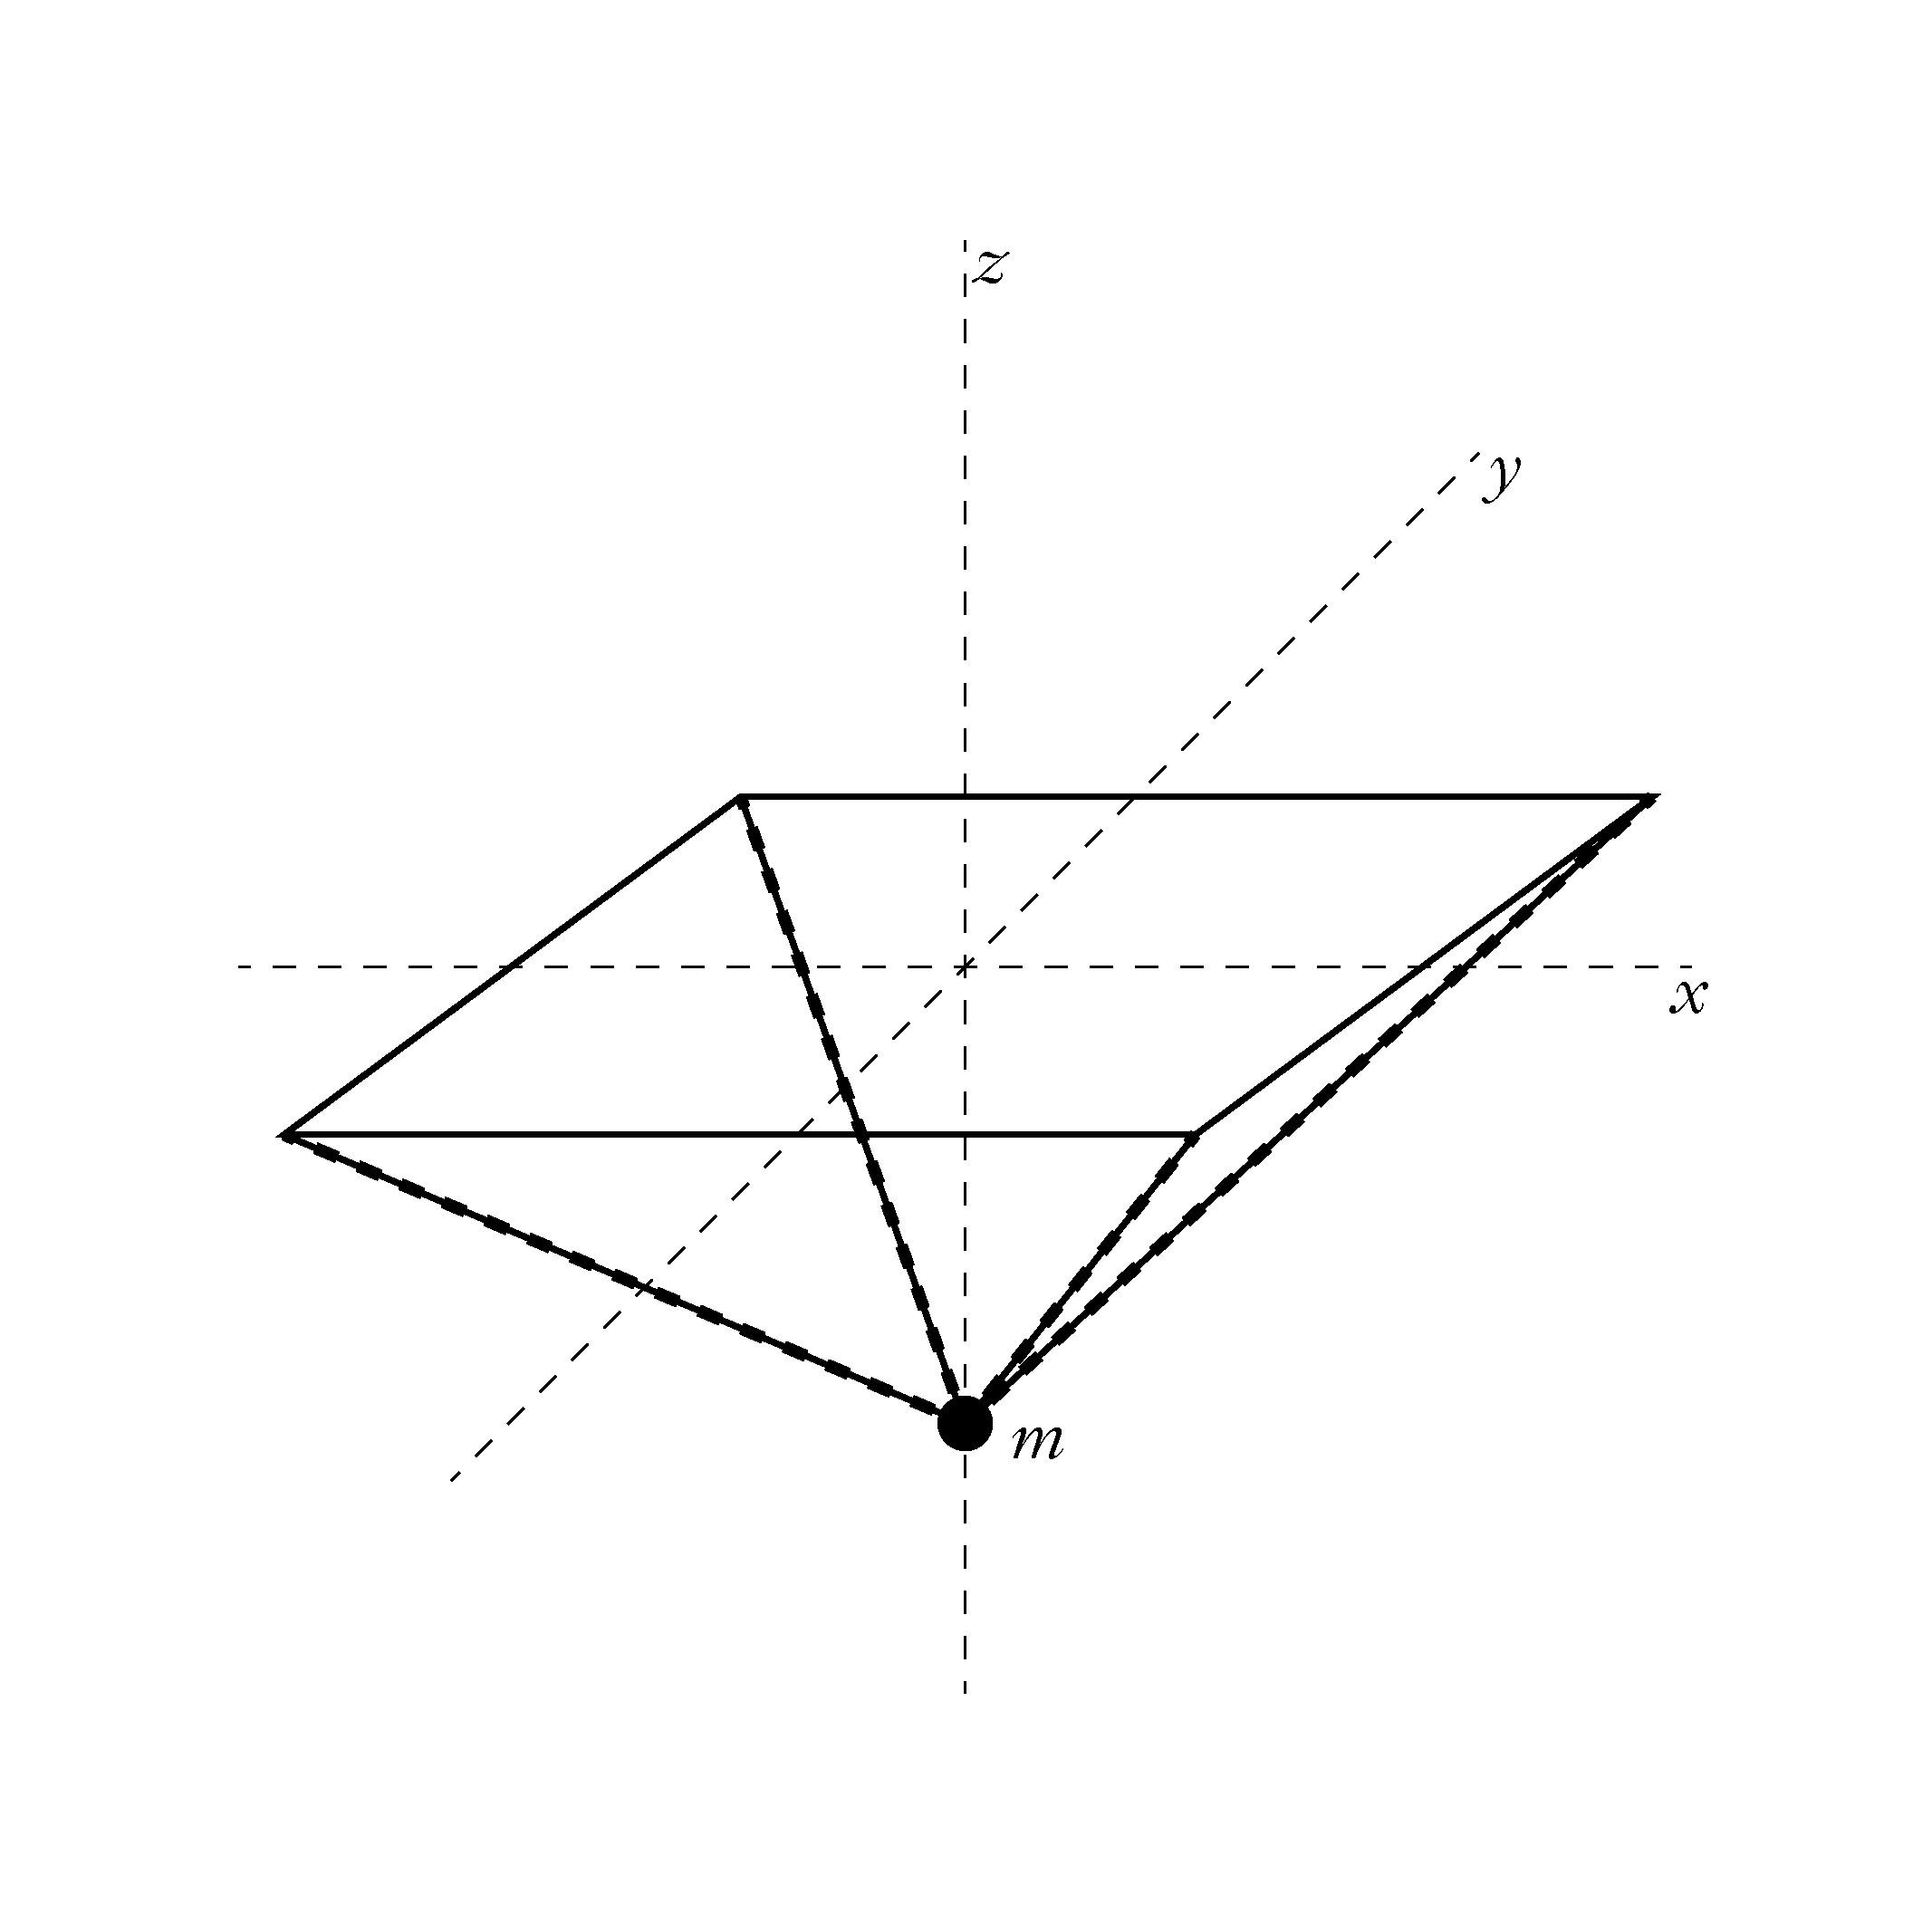
\includegraphics[height=1.3in]{plot.pdf}
%\end{center}

% \blindtext \cite{article-minimal}

% \bibliographystyle{apsrev4-1} % Tell bibtex which bibliography style to use
% \bibliography{xampl} % Tell bibtex which .bib file to use (this one is some example file in TexLive's file tree)

\end{document}